\documentclass[tikz,border=8pt]{standalone}
\usepackage{amsmath}
\usetikzlibrary{arrows.meta}
\begin{document}
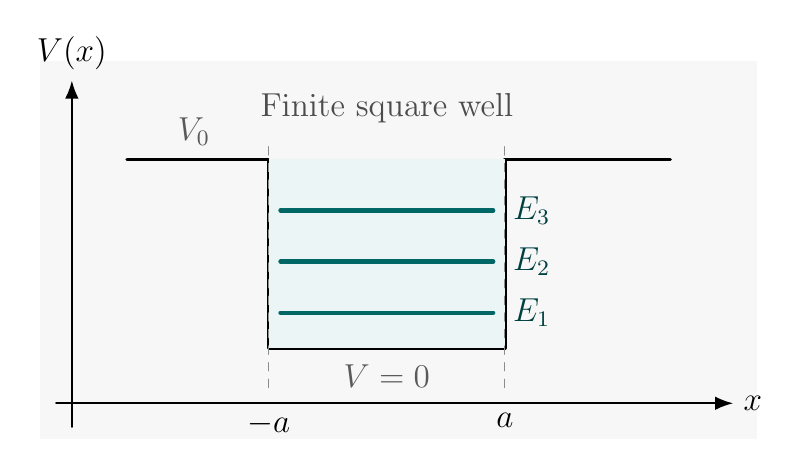
\begin{tikzpicture}[>=Latex, line cap=round, line join=round, font=\large]
  \fill[black!3] (-4.4,-.45) rectangle (4.7,4.35);
  \draw[->, thick] (-4.2,0) -- (4.4,0) node[right] {$x$};
  \draw[->, thick] (-4,-.3) -- (-4,4.1) node[above] {$V(x)$};
  \draw[very thick, black] (-3.3,3.1) -- (-1.5,3.1) -- (-1.5,.7) -- (1.5,.7) -- (1.5,3.1) -- (3.6,3.1);
  \fill[teal!8] (-1.5,.7) rectangle (1.5,3.1);
  \foreach \y/\name in {1.15/E_1,1.8/E_2,2.45/E_3} {
    \draw[teal!80!black, ultra thick] (-1.35,\y) -- (1.35,\y);
    \node[teal!50!black, right] at (1.48,\y) {$\name$};
  }
  \draw[dashed, black!45] (-1.5,.2) -- (-1.5,3.35);
  \draw[dashed, black!45] (1.5,.2) -- (1.5,3.35);
  \node[below] at (-1.5,0) {$-a$};
  \node[below] at (1.5,0) {$a$};
  \node[black!65] at (0,.35) {$V=0$};
  \node[black!65] at (-2.45,3.45) {$V_0$};
  \node[align=center, black!70] at (0,3.75) {Finite square well};
\end{tikzpicture}
\end{document}
